% NOTE (migration 23 Nov 2026): Text moved unchanged from main.tex. Much of it was drafted with AI assistance; rewrite it in your own words before submission (the supervisor runs AI checks).
% NOTE (24 Nov 2026): Section evidence-llm added from thesis/evidence/2026-11-23-full and 2026-11-24-contract (drafted with AI assistance; reword before submission).
\chapter{Results}\label{evidence}

\section{Purpose and boundary}
This chapter records measured evidence about the implemented JadwAI system between 8 and 28 November 2026. It concerns the scheduling engine, its independent validator, the repair diagnosis for impossible timetables, reports and exports, a supervisor-style test of all four timetables, a comparison with a real GIU timetable, and the interpretation results of the rule-based parser and the local language model on the development corpus (RQ1, RQ2). The interpretation results are development-level evidence: the corpus labels remain draft and unreviewed (Section~\ref{dataset-construction}), and no paid provider was used. Engineering checks and research results are kept separate. Section~\ref{evidence-jai-results} reports the evaluation of the JAI assistant and the fine-tuning of its locally hosted model (described in Section~\ref{evidence-jai}); those measurements concern assistant behaviour on development cases, not the constraint-extraction questions.

All runs used one laptop (Intel Core i5-1038NG7, 4~cores and 8~threads, 16\,GB memory, macOS~26.5.1), Python~3.14.5 and OR-Tools CP-SAT~9.15.6755~\cite{google_cpsat} with eight search workers and random seed~42. Times are wall-clock seconds on that machine and depend on hardware. Every timetable reported as valid passed JadwAI's independent validator, which recomputes completeness, eligibility, the doctor/TA split, room suitability and capacity, resource overlaps, approved rules, locks, workload and daily policies without using the solver's model. The code is at commits \texttt{e4771a1} and \texttt{4137b96} of the project repository plus the parser correction described in Section~\ref{evidence-baseline}. Scripts and logs are kept in \texttt{thesis/evidence/2026-11-08/}.

\section{Teaching timetable at department scale}\label{evidence-department}
The demonstration workspace contains 448 weekly sessions, 93 student groups in eight programmes, 123 instructors, 65 rooms and 60 advising students (students whose courses differ from their group's, for example a retake, a section change or an elective from another programme). The calendar has six teaching days with five 90-minute periods, a student limit of 7.5 teaching hours per day and at most four consecutive periods.

\begin{itemize}
\tightlist
\item \textbf{One run.} Generation with the convenience objective completed in 253\,s and passed independent validation. None of the 60 advising students has two of their own sessions at the same time. Evaluated on the same timetable without modelling them, 24 of the 60 would have had a clash.
\item \textbf{Published draft.} A later run (222.9\,s) placed all 448 sessions with zero room, instructor and group overlap pairs. All 65 rooms are used by more than one programme, so the absence of room double-booking is a cross-programme property rather than a per-programme one. Room time used was 23.0\% and seats filled 66.2\%, counting advising students who join or drop sessions. Part of this timetable is shown in Figure~\ref{fig:shot-teaching-timetable-2} (Appendix~\ref{app:screenshots}).
\item \textbf{Two parts.} Built as Applied Computer Science and Informatics (217 sessions) followed by the remaining seven programmes (231 sessions) with the first part fixed, the parts took 128\,s and 129\,s, each passed validation as a combined timetable, and only the complete draft could be published.
\end{itemize}

\section{Teaching timetable at university scale}\label{evidence-university}
The Winter 2026 workbook, entered through the data template, yields 2{,}711 weekly sessions for 349 groups, 669 staff and 65 rooms. This exceeds the 600-session limit of a single run, so the timetable is generated in parts of one or more programme years, each part placed around the fixed sessions of earlier parts (Engineering alone has 912 sessions).

\paragraph{What the input checks found.} Before any search, the input checks identify why the data as entered cannot produce a timetable:
\begin{itemize}
\tightlist
\item 23 of 446 teaching assistants cannot be given an activity of their own, contradicting the rule that every TA teaches;
\item eight lectures for 300--350 students have no room large enough;
\item sessions needing laboratories require 1{,}160 teaching hours a week, while the 18 laboratories provide 810; lecture and tutorial sessions require 2{,}907 hours against 2{,}115;
\item two courses (X118 and ENGN101) each need 87 hours a week from two TAs who have 75 hours between them;
\item every Engineering Year~3 group needs 34.5 of the 36 hours its week can hold under the daily limits (a near-full week rather than an impossibility).
\end{itemize}
The TA names in the entered workbook are placeholders and the 65 rooms appear to cover one building, so these findings describe the entered data rather than the university.

\paragraph{Generation in parts with documented adjustments.} To test the part mechanism at full scale, the experiment set aside the eight oversized lectures and the 23 idle TAs, added 32 placeholder TAs (so no TA pool exceeds half its capacity) and 86 placeholder rooms (25 laboratories, 61 lecture rooms; about 60\% room load), and switched off the daily policies. Table~\ref{tab:parts} reports the result with 120\,s per part.

\begin{table}[h]
\centering
\small
\begin{tabular}{@{}rrrrl@{}}
\toprule
Part & New sessions & Scheduled so far & Time (s) & Validation \\
\midrule
1 & 328 & 328 & 125 & passed \\
2 & 584 & 912 & 127 & passed \\
3 & 572 & 1{,}484 & 127 & passed \\
4 & 581 & 2{,}065 & 128 & passed \\
5 & 598 & 2{,}663 & 130 & passed \\
6 & 40 & 2{,}703 & 128 & passed \\
\bottomrule
\end{tabular}
\caption{University-scale teaching timetable built in six parts (adjusted data; see text).}
\label{tab:parts}
\end{table}

Every earlier session was unchanged in each later part, and the final timetable also passed validation as one whole timetable without the part plan. Two observations qualify the result. First, with the daily policies switched on, Engineering Year~3 alone found no timetable within 300\,s, while without them it was solved in 3\,s; this is consistent with the near-full week reported above. Second, convenience is optimised within each part around fixed sessions, so earlier parts are never improved by later ones; the order of parts matters.

\section{Comparison with a real GIU timetable}\label{evidence-real}
The university's staff planning for Spring 2024 and the timetable that was published from it (version~17 of the Spring 2024 schedule) were made available for this comparison with the supervisor's agreement. The staff planning lists, per faculty, each course with its cohorts, weekly lecture, tutorial and laboratory hours, numbers of lecture and tutorial groups, lecturer and number of teaching assistants. The published timetable is a grid for people: one sheet per day, a row per cohort and stream, and five periods per day. Only aggregate figures are reported here; no staff names are used.

\paragraph{Input.} A loading script read the staff planning into an empty workspace. Following the owner's interpretation, an hour is 60 minutes and a session is 90 minutes, so each activity receives the nearest whole number of sessions (at least one); a 2-hour tutorial therefore becomes one session. This gives 188 courses, 269 student groups in 54 cohorts, 1{,}183 activities and 1{,}489 weekly sessions (234 lecture, 672 tutorial, 583 laboratory), with 134{,}010 scheduled minutes against 158{,}940 planned (16\% fewer). Teaching assistants are not named in the staff planning, so 256 placeholder TAs were created; 29 courses without a named lecturer received a placeholder lecturer. The real room list was not available: the 65 rooms of the demonstration workspace were used, plus 17 marked placeholder rooms (large halls and laboratories), because 189 lecture sessions need more than 35 seats and 583 laboratory sessions compete for 15 laboratories. The week is Saturday to Thursday with five periods from 08:30 to 17:15.

\paragraph{Runs.} The 1{,}489 sessions exceed the size of a single run, so both runs were built automatically in five parts (Section~\ref{evidence-university}) of about four minutes each. All sessions were placed and each run passed independent validation. Run~1 used no further rules. In the real timetable each cohort has fixed days off; run~2 added them as 278 approved group-unavailable rules covering the whole day, and changed nothing else.

\paragraph{Method.} The grid has no stable course codes, so sessions were compared at the level of cohort (faculty and semester), student group, day and period rather than one session against another. A cell counts once for each period it covers. German and English language classes (103 cells) are not in the staff planning and were left out, leaving 1{,}555 teaching cells. For the course-level comparison, course names in the grid (often abbreviated, such as ``CS~II'' or ``RM'') were matched to staff-planning names within the same cohort by abbreviation, initials and Roman numerals: 1{,}208 of 1{,}297 cells in cohorts with a semester (93\%) matched one of 143 course--cohort pairs. Most unmatched cells are misspelt in the grid or name courses that are not in the staff planning.

\paragraph{Effect of the days off.} Without days off, JadwAI spread every cohort over all six days: cohorts taught on 5.2 days on average against 4.3 in the real timetable, and 78 of 267 groups (29\%) came to campus every day against none. With the days off (run~2), every cohort has the same number of teaching days as in the real timetable, five groups (2\%) come every day, all in a 6th-semester cohort that also has no day off in reality, and the share of teaching per weekday matches within one percentage point (Saturday 11\% and Thursday 13\% in both). The remaining figures refer to run~2.

\begin{table}[h]
\centering
\small
\begin{tabular}{@{}lrr@{}}
\toprule
 & Real & JadwAI (run 2) \\
\midrule
Student groups compared & 250 & 267 \\
Teaching days per cohort (mean) & 4.3 & 4.3 \\
Days on campus per group (mean) & 3.6 & 3.8 \\
Groups on campus all six days & 0 & 5 \\
Empty periods between classes per group and week (mean) & 0.9 & 0.5 \\
Groups with no empty periods & 49\% & 68\% \\
Sessions at 08:30 or 15:45 & 24\% & 16\% \\
Rooms in use per period (mean / peak) & 40 / 63 & 50 / 82 \\
\bottomrule
\end{tabular}
\caption{JadwAI run~2 and the published Spring 2024 timetable, both built from the same staff planning. Real room counts are the grid's own summary rows; JadwAI counts distinct rooms.}
\label{tab:real}
\end{table}

\paragraph{Results.} Table~\ref{tab:real} summarises the comparison. The weekly shape of each cohort is close to the real one: the cosine similarity of the cohorts' sessions per day averages 0.90 (1 is identical), and 0.66 per day and period. Course by course, on average 69\% of the days a course has in the real timetable are also days JadwAI uses for it (all of them for 59 of 143 courses, none for 17), but only 31\% of the real (day, period) slots are the same, and 41 courses share no slot at all. Random placement would share about 17\% of days and 3\% of slots, so the overlap is not chance, yet JadwAI does not reproduce the real timetable, and it was not asked to: many different timetables satisfy the same planning. The largest differences are in 6th-semester electives, where JadwAI is free to choose among many valid days. JadwAI leaves fewer empty periods between classes and uses the first and last periods less, which follows from its convenience objective. It uses more rooms at the same time, partly because the placeholder rooms (used in 320 of 1{,}489 session-periods) make more rooms available than the real campus offers in this model.

\paragraph{Limits.} The real figures per group are read from cell text, which is not always consistent; lectures without a group number are counted for every group of their stream. Design and Physical Therapy are only partly comparable because their grid layout differs from the staff planning (Design has 258 real teaching cells against 116 JadwAI session-periods). The rule ``nearest whole number of 90-minute sessions'' schedules 16\% fewer minutes than planned. Rooms, TAs and some lecturers are placeholders, and real room features and capacities were not modelled, so room figures are not comparable in detail. The days off were copied from the real timetable rather than derived by JadwAI. The comparison therefore shows that JadwAI produces a complete, valid timetable of the same scale and weekly shape from the university's own planning; it does not show that it is better or worse than the published timetable, which reflects constraints that were not available here.

\section{Examination timetable}
For all 203 courses of the workbook, the examination model first computes a proven lower bound on the number of back-to-back examination days that any timetable over the given dates must contain (372). It reached that bound within 20\,s; the previous formulation found no timetable within 20\,s and 423 back-to-back days within 120\,s. Allowing two examinations per day reduced back-to-back days to 302 at the cost of 35 days with two examinations; adding four examination dates reduced them to 51. In the demonstration workspace, 35 examinations over ten days were scheduled in halls with TA invigilators; no advising student has two examinations at the same time, and the one student whose courses cannot be spread further within the dates is named for the administrator.

\section{Repair suggestions for impossible timetables}\label{evidence-repair}
When the approved inputs cannot all hold, JadwAI relaxes what an administrator could change---each approved rule, each fixed session, each instructor's day off and each daily limit---and restores them a chunk at a time while a timetable still exists. The remaining set is minimal (no single member can be restored), not necessarily the smallest possible. The affected sessions are reported from a repaired timetable that the independent validator checks against everything else. Physical data limits (rooms, eligible instructors, ``every TA teaches'', the calendar) are never relaxed. Table~\ref{tab:repair} lists the deliberately impossible cases tested.

\begin{table}[h]
\centering
\small
\begin{tabular}{@{}p{0.42\textwidth}p{0.48\textwidth}@{}}
\toprule
Injected problem & Diagnosis \\
\midrule
Two sessions of one group locked to the same time & Move one session; new day, time and room given; verified \\
The only eligible instructor unavailable all week & Relax that rule; the one affected session listed; verified \\
Instructor's day off is the group's only free day & Either the day off or the group rule (one change); verified \\
Daily limit of 2 hours with 4 hours of teaching in one day & Relax the limit; ``needs 4\,h on Sunday''; verified \\
Two courses on separate days with one teaching day & Relax the rule; both sessions listed; verified \\
Five teaching hours in a four-hour week & No relaxation helps; data must change; overloaded group named \\
\midrule
Demonstration (448 sessions): an instructor unavailable all week and a G7 session locked inside the group's blocked time & Exactly these two causes, the locked session moved to another slot; 49\,s, 19 feasibility solves, 138 sessions examined locally, verified on the whole timetable \\
\bottomrule
\end{tabular}
\caption{Repair diagnosis on impossible timetables.}
\label{tab:repair}
\end{table}

On timetables above 80 sessions a complete diagnosis is too slow (one feasibility solve on the 448-session workspace takes 18--73\,s), so the search starts with the sessions the failure points at and those sharing a group or instructor with them, then proves the fix on the whole timetable within a 240\,s budget. An early version kept a limit that was not needed because a five-second check had ended without a result; inconclusive checks are now retried with more time before a candidate is declared necessary. An inconclusive search is never reported as proof.

\section{Rule-based interpretation baseline}\label{evidence-baseline}
Section~\ref{baselines} describes the two interpretation methods compared for RQ1 and RQ2. JadwAI's built-in parser (deterministic patterns for English, formal Arabic and Egyptian Arabic) was run on all 144 statements of the development release (36 intent families, four language variants each) and scored with the project's offline scorer, which validates each output against the contract and the synthetic context before comparing it with the expected answer. The parser received only entity names as stored in JadwAI (English), not the context's Arabic aliases. A format adapter wrote whole hours as integers (10 rather than 10.0), which the contract requires; half-hour values were left unchanged.

The parser was measured twice. The first measurement exposed that its clarification codes differed from annotation guide~v2 and that it guessed in three situations where the guide requires a question. The parser was then changed, and the second measurement is the one reported in Table~\ref{tab:baseline}. The changes were: (1)~clarification codes renamed to the guide's stable codes (for example \texttt{ambiguous\_instructor} instead of \texttt{ambiguous\_name:ahmed}, and \texttt{unknown\_instructor}); (2)~a mandatory time without a day, a statement naming no rule type (``Nour Hassan, Sunday, 08:00--10:00''), and vague times such as ``early'' now produce questions (\texttt{day\_required}, \texttt{rule\_type\_and\_strength\_required}, \texttt{undefined\_early}) instead of an assumed interpretation; (3)~common Egyptian and English negations that were missing (for example the Egyptian equivalents of ``not available'' and ``cannot'', and ``do not schedule'') were added, together with ``must fit'' and ``no other times''; and (4)~``Monday and Tuesday \ldots{} on each day'' is read as those two days rather than every day. Change~(3) mattered for safety: before it, a statement such as ``Nour Hassan [not available] Sunday 08:00--10:00'' fell through to the ``only'' interpretation and produced the opposite rule. Because these changes were made after inspecting development errors, the reported figures are optimistic for this release and are not evidence of performance on unseen statements.

\begin{table}[h]
\centering
\small
\begin{tabular}{@{}lrrl@{}}
\toprule
Measure & First run & Reported & 95\% interval (reported) \\
\midrule
End-to-end exact output & 0.153 (22/144) & 0.326 (47/144) & 0.215--0.458 \\
Decision accuracy & 0.521 & 0.597 & 0.465--0.736 \\
Proposal precision / recall & 0.222 / 0.315 & 0.448 / 0.361 & \\
Proposal F1 & 0.261 & 0.400 & 0.295--0.515 \\
Field F1 & 0.451 & 0.605 & 0.474--0.712 \\
Clarification F1 & 0.000 & 0.351 & 0.141--0.576 \\
Unsupported-request F1 & 0.000 & 0.000 & \\
\bottomrule
\end{tabular}
\caption{Rule-based baseline on the draft development labels before and after aligning the parser with annotation guide~v2 (intervals: percentile bootstrap over intent families, 1{,}000 replicates).}
\label{tab:baseline}
\end{table}

In the reported run, exact outputs by language were 20/36 (English), 12/36 (mixed), 8/36 (formal Arabic) and 7/36 (Egyptian Arabic); decision accuracy was 0.69, 0.67, 0.53 and 0.50 respectively, and all 144 outputs were contract-valid. Unsupported-request F1 remains zero for two reasons: the parser has no proposals for weekly teaching loads or locks (12 expected), and it deliberately differs from guide~v2 on minute-precise times. The guide labels a closure such as 10:15--11:45 as unsupported; the application stores half hours and rounds closures outwards (10:00--12:00), which suits the 15--30-minute breaks between the institution's teaching periods. This is a recorded design difference, not an error in either. Because the labels are draft and unreviewed, the families are synthetic and the release is development material, these figures describe a baseline on development data only; they are not a confirmatory result. The language model is compared in Section~\ref{evidence-llm}.

Testing the interpretation workflow on the demonstration workspace also found three faults that were then corrected: a closure ending at 15:15 was stored as ending at 15:00 (closures are now rounded outwards and permitted or preferred windows inwards); the review editor could not show a 10:30 interpretation (it now offers half hours); and Arabic statements could not name instructors stored in English (names are now compared by consonant sounds in both scripts, with Egyptian and classical readings, and a shared first name triggers a clarification).

\section{Local language model interpretation}\label{evidence-llm}
The local model (Section~\ref{baselines}) was run on the same 144 development statements twice: first with the application's own prompt, then with a prompt written for the evaluation contract. Both runs used the same model, schema order and decoding settings, and were scored with the same scorer and adapter as the parser. Table~\ref{tab:llm} and Figure~\ref{fig:llm} compare the three results. The data, predictions, logs and analyses are in \texttt{thesis/evidence/2026-11-23-full/} and \texttt{thesis/evidence/2026-11-24-contract/}.

\begin{table}[h]
\centering
\small
\begin{tabular}{@{}lp{0.17\textwidth}p{0.17\textwidth}p{0.17\textwidth}@{}}
\toprule
Measure & Rule-based parser & Model, application prompt & Model, contract prompt \\
\midrule
Exact output & 0.326 (47) \newline 0.215--0.458 & 0.090 (13) \newline 0.028--0.167 & 0.167 (24) \newline 0.069--0.264 \\
Decision accuracy & 0.597 \newline 0.465--0.736 & 0.479 \newline 0.340--0.604 & 0.556 \newline 0.431--0.674 \\
Contract-valid outputs & 144 & 18 & 122 \\
Proposal precision / recall & 0.448 / 0.361 & 0.116 / 0.204 & 0.169 / 0.407 \\
Proposal F1 & 0.400 & 0.148 & 0.239 \\
Field F1 & 0.605 & 0.313 & 0.380 \\
Clarification F1 & 0.351 & 0.000 & 0.104 \\
Unsupported-request F1 & 0.000 & 0.000 & 0.160 \\
Unknown entities (cases) & 0 & 16 & 6 \\
Median seconds per statement & --- & 116 & 39 \\
\bottomrule
\end{tabular}
\caption{Interpretation of the 144 development statements by the parser and by the local model with two prompts (95\% percentile bootstrap intervals over the 36 intent families, 1{,}000 replicates, seed~42).}
\label{tab:llm}
\end{table}

\begin{figure}[t]
\centering
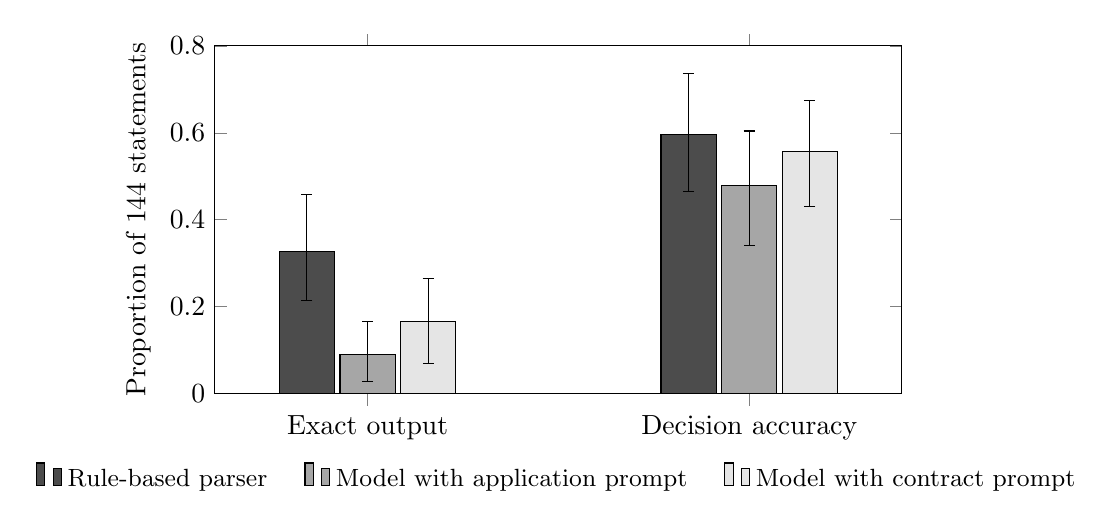
\begin{tikzpicture}
\begin{axis}[
  ybar, bar width=7mm, width=0.85\textwidth, height=6cm,
  ymin=0, ymax=0.8, ylabel={Proportion of 144 statements},
  symbolic x coords={Exact output, Decision accuracy}, xtick=data,
  enlarge x limits=0.4, legend style={at={(0.5,-0.18)}, anchor=north, legend columns=-1, draw=none, font=\small, /tikz/every even column/.append style={column sep=4mm}},
  error bars/y dir=both, error bars/y explicit]
\addplot[fill=black!70] coordinates {(Exact output,0.326) += (0,0.132) -= (0,0.111) (Decision accuracy,0.597) += (0,0.139) -= (0,0.132)};
\addplot[fill=black!35] coordinates {(Exact output,0.090) += (0,0.077) -= (0,0.062) (Decision accuracy,0.479) += (0,0.125) -= (0,0.139)};
\addplot[fill=black!10] coordinates {(Exact output,0.167) += (0,0.097) -= (0,0.098) (Decision accuracy,0.556) += (0,0.118) -= (0,0.125)};
\legend{Rule-based parser, Model with application prompt, Model with contract prompt}
\end{axis}
\end{tikzpicture}
\caption{Exact output and decision accuracy of the three interpretation methods on the development statements. Error bars are the 95\% intervals from Table~\ref{tab:llm}; those of the parser and of the model with the contract prompt overlap.}
\label{fig:llm}
\end{figure}

\paragraph{First run: application prompt.} Only 18 of the 144 outputs passed the contract check. The main reason was a mismatch between the application and the evaluation contract, not only the model. The application's prompt had been extended after the contract was fixed in October: it describes rule types such as preferred teaching windows and daily teaching limits, and a parameter field, which the contract does not know. The model used them in 56 proposals. The prompt also did not list the guide's clarification codes, so the model invented its own (for example \texttt{clarify\_if\_needed}), and clarification F1 was zero. Decisions are scored separately from the vocabulary, and they show a real behaviour: the model mostly answered \texttt{ready}. It treated 24 of 44 statements that need a question, all 8 conflicts and 11 of 16 unsupported requests as ready, and it referred to identifiers that were not in the context in 16 cases.

\paragraph{Second run: contract prompt.} With the contract's vocabulary and codes in the prompt, 122 outputs were valid and exact output nearly doubled, from 13 to 24. The model now asked more often: it recognised 25 of the 44 statements that need a question, against 5 in the first run, but it also asked in 16 of 76 clear statements. Exact outputs by language were 8 (English), 8 (formal Arabic), 3 (Egyptian Arabic) and 5 (mixed) of 36. Three errors remained:
\begin{itemize}
\item \emph{Wrong rule kind.} The model produced 161 weekly-limit proposals where the labels have 8. In 57 of them it represented a day-specific unavailability (``cannot teach Sunday 08:00--10:00'') as a weekly limit of zero hours, which the prompt's phrase ``0 forbids teaching'' probably invited; in 79 it added a 12-hour limit that the statement did not mention. This explains why recall rose to 0.41 while precision stayed at 0.17.
\item \emph{Conflicts.} None of the 8 conflicting statements was recognised; 5 of them produced no valid output.
\item \emph{Invalid replies.} The 12 invalid replies each took 330 to 383 seconds and contained no complete JSON, which suggests that the model reached the output limit while generating.
\end{itemize}

\paragraph{Comparison with the parser.} The parser remained higher on every measure except unsupported requests, where it scores zero by design (Section~\ref{evidence-baseline}). The intervals of the parser and of the second model run overlap for exact output and decision accuracy, so these 144 statements cannot show a reliable difference on those two measures; the parser's advantage in proposal and field F1 is clearer. Both methods were adjusted on the same development data, the parser after its first run and the model prompt by writing the code meanings from the labels, so neither figure is an estimate for unseen statements.

\paragraph{A label inconsistency.} Writing the code list for the second prompt showed that the draft labels use two codes for a missing day (\texttt{day\_required} and \texttt{missing\_day}) and two for minute-precise rules. A method cannot know which of two synonyms is expected, so a few clarification and unsupported errors of both methods are noise in the labels. The labels were not changed for these runs; the codes should be merged before the labels are reviewed.

\section{Automated check of the draft labels}\label{evidence-labelcheck}
The interpretation results above rely on draft labels that no human has reviewed (Section~\ref{dataset-construction}). A human audit of a stratified sample was prepared but not carried out. Instead, all 144 labels of the 0.2.1 bundle (guide~v2.1) were checked automatically on 28 November 2026. This is a consistency check, not a review: it was written and run by the same AI assistant that drafted the labels and the guide, so it shares their blind spots, and the labels keep the status ``draft, unreviewed''.

\paragraph{Mechanical checks.} A script checked every label for: a decision that matches its content (for example, \texttt{ready} with at least one proposal and no codes); clarification and unsupported codes that are current guide codes; instructor, room, group and activity IDs that exist in the context; days inside the context's week; whole hours inside the teaching day; hard strength for closures and soft strength for preferences; locks that point at the context draft; clock times in the English statement that match the proposal hours; one label shared by all four translations of a family; and the same codes for families with the same proposal pattern. Deliberately broken labels were used to confirm that each check fires. No label failed a check, and the four translations of every family carry the same label. One pattern check failed: \texttt{family-022} and \texttt{design-family-012} describe the same situation (a course whose only permitted window is fully covered by a closure of its group) but use different clarification codes, \texttt{hard\_window\_has\_no\_placement} and \texttt{resolve\_hard\_conflict}.

\paragraph{Reading against the guide.} The assistant also read each of the 36 families against the guide. It agreed with 33. The two families above disagree with each other; as with the synonyms merged in guide~v2.1 (Section~\ref{evidence-llm}), a method cannot know which code is expected, so one of the two should change. One family is ambiguous: \texttt{design-family-009} (``Studio~2 is closed on Saturday from 10:15 to 11:45'') is labelled unsupported because manual rules store whole hours, but unlike \texttt{family-020} it does not ask for exact times, and a 10:00--12:00 closure blocks exactly the same teaching period; the application's own outward rounding (Section~\ref{evidence-baseline}) would accept it. Three further notes concern wording only: two Arabic group names are paraphrases rather than context aliases, one formal Arabic statement says ``lectures'' where the others say ``classes'', and one statement lacks a day as well as a definition of ``early''. Together the three flagged families contain 12 of the 144 labels.

\paragraph{What it supports.} The check supports the statement that the draft labels are internally consistent, apart from one pair of families with different codes and one ambiguous family. It does not show that the labels are correct, and it is not independent or double annotation. No label was changed; a correction belongs in a new bundle version with a correction log.

\section{Reports and exports}
The statistics report for the published draft was recomputed independently from the saved assignments; every figure matched (448/448 sessions, sessions per day, zero overlaps, 65/65 rooms, 123/123 instructors, 22.97\% room time, no extra teaching hours). The review found that seat use ignored advising students, that unset limits were printed as ``None'', and that a report could not be limited to one group; all three were corrected. Timetable PDFs are now generated on the server as landscape A4 pages with short descriptive names (for example ``BA Y3 G7 Schedule'') because browser printing in one environment rotated the page and named the file after the application window.


\section{The JAI assistant: evaluation}\label{evidence-jai-results}

\paragraph{Automatic checks on held-out cases.} Each candidate answered the same held-out cases with the production prompt, at temperature~0. The automatic checks cover only whether the reply is valid, whether it wrongly proposes an action, whether it is in the user's language and whether it stays under 80 words; they do not judge correctness. Table~\ref{tab:jai-auto} reports the conversation cases with the guide in the prompt.

\begin{table}[h]
\centering
\small
\begin{tabular}{@{}lrrrrr@{}}
\toprule
16 held-out conversation cases & Base & v1 & v2 & v3 & v4 \\
\midrule
Valid reply & 16 & 16 & 16 & 16 & 16 \\
No wrongly proposed action & 15 & 16 & 15 & 16 & 16 \\
Reply in the user's language & 16 & 13 & 12 & 14 & 14 \\
At most 80 words & 14 & 16 & 12 & 14 & 16 \\
\midrule
Action choice (5 separate cases) & 3 & 5 & 5 & 4 & 5 \\
\bottomrule
\end{tabular}
\caption{Automatic checks. Base, v1 and v2 were run on 22 November; v3 on 23 November with the extended guide, where v1 re-run on identical prompts gave 13 replies in the user's language and 16 under 80 words; v4 on 24 November with the same prompts as v3.}
\label{tab:jai-auto}
\end{table}

Round~2 is a negative result worth recording. Its training answers had been written before the guide existed and were left unchanged when the guide was added to the prompts, so the model was trained to receive the guide and then answer in its own words; it invented more than v1 (``snapshots on the cloud'', solver settings that do not exist). Lower training loss with an extra epoch reflected memorisation of 210 rows rather than better answers. Round~3 rewrote the answers so that every statement about JadwAI comes from the guide entries present in that example's prompt, and the dataset builder now refuses an example whose prompt lacks the guide entries its answer relies on.

\paragraph{Blind human rating.} For v1 and v3, the 19 held-out conversation answers (16 cases and three wordings of a new ``not sure'' question) were placed side by side in random order, without model names, and scored from 1 to 5 on correctness, logic, helpfulness and natural language (Table~\ref{tab:jai-rating}). The rater was the project owner, who had read a short summary of some replies beforehand, so the rating is neither independent nor fully blind.

\begin{table}[h]
\centering
\small
\begin{tabular}{@{}lrr@{}}
\toprule
19 cases, 4 criteria, 1--5 each & v1 & v3 \\
\midrule
Total (maximum 380) & 244 & 274 \\
Mean per case (maximum 20) & 12.8 & 14.4 \\
Correct / logical / helpful / natural (means) & 3.3 / 3.3 / 3.1 / 3.2 & 3.7 / 3.6 / 3.6 / 3.5 \\
Cases won (8 ties) & 3 & 8 \\
\bottomrule
\end{tabular}
\caption{Blind side-by-side rating of fine-tuned v1 and v3.}
\label{tab:jai-rating}
\end{table}

The largest gains were in Arabic: an Arabic privacy question that v1 answered in English, and a request for ``no classes at 08:30'' that v1 answered by claiming such classes were forbidden, while v3 correctly said no mandatory rule prevents them. Six cases received the minimum score for both models, including an off-topic request for a poem and an Arabic question about shared lectures.

\paragraph{Live use.} With v3 in the running application, four questions taken from the weakest cases were asked in the chat. The display of mixed Arabic and English text was correct after the fix described in Section~\ref{evidence-jai}, but the answers were weak: an Arabic question about laboratories with GPUs used wrong words for rooms; the poem request produced a poem; a frustrated Arabic message drifted into Chinese mid-sentence; and a question about connecting to the university's student information system, asked after the complaint, was answered with a request for a rule identifier from the previous topic. The held-out measurements therefore overstate live reliability, particularly for topic changes within one conversation. These cases were used to write a fourth round of training examples (off-topic requests, topic changes, Arabic room vocabulary and examination publishing), which were trained as round~4 (v4; Table~\ref{tab:jai-rounds}).

\paragraph{Round 4.} On the old held-out cases v4 matched v3 on validity, actions and language, kept every reply under 80 words and chose the examination timetable correctly in the action case that v3 had missed (Table~\ref{tab:jai-auto}); it was also about 12\% faster per answer. Round~4 also held out one new family for each live failure, 13 cases in total, which neither model had seen (Table~\ref{tab:jai-round4}).

\begin{table}[h]
\centering
\small
\begin{tabular}{@{}lrr@{}}
\toprule
13 new held-out cases (4 families) & v3 & v4 \\
\midrule
Right action (none, or the expected one) & 10 & 9 \\
Reply in the user's language & 9 & 10 \\
At most 80 words & 12 & 13 \\
Mentions an internal API path & 1 & 2 \\
\bottomrule
\end{tabular}
\caption{Round-4 held-out families: off-topic story (3), changing topic from a rule to the portal (3), adding a laboratory with GPUs (4) and a formal request to publish the examination timetable (3).}
\label{tab:jai-round4}
\end{table}

These automatic differences are within one or two cases and do not by themselves show that v4 is better. Reading the replies shows where it changed. Both models declined the English story requests; in Arabic, v3 drifted into a long, repetitive timetable summary, while v4 stayed short but mixed in an English phrase. For the English GPU questions v4 gave the right steps (add a room with the laboratory type and the GPU feature), where v3 asked which room was being replaced. Neither model answered the Arabic GPU questions in Arabic, and v4 quoted an internal API path in both of them. Neither model turned ``publish the exam schedule'' in conversation into the publish action in any of the three cases, so the examination examples in round~4 did not fix the failure they targeted. The project owner then rated v3 and v4 side by side on all 32 cases (the 19 earlier cases and the 13 new ones) in the same way as before, again after reading a summary of the automatic results and some replies (Table~\ref{tab:jai-rating-v4}).

\begin{table}[h]
\centering
\small
\begin{tabular}{@{}lrr@{}}
\toprule
32 cases, 4 criteria, 1--5 each & v3 & v4 \\
\midrule
Total (maximum 640) & 461 & 524 \\
Mean per case (maximum 20) & 14.4 & 16.4 \\
Correct / logical / helpful / natural (means) & 3.5 / 3.6 / 3.6 / 3.7 & 4.0 / 4.1 / 4.1 / 4.2 \\
Earlier 19 cases / new 13 cases (totals) & 293 / 168 & 317 / 207 \\
Cases won (12 ties) & 6 & 14 \\
\bottomrule
\end{tabular}
\caption{Blind side-by-side rating of fine-tuned v3 and v4. Scores from different sheets are not comparable: v3 received 293 here and 274 on the same 19 cases in Table~\ref{tab:jai-rating}.}
\label{tab:jai-rating-v4}
\end{table}

The rating favoured v4 on both the earlier and the new cases, unlike the automatic checks. The largest differences were an off-topic request for a poem (4 against 20 points), which v3 did not decline, the Arabic story request (8 against 20) and the Arabic portal question (10 against 20). v4 lost most clearly on an Arabic question about special rooms (14 against 10) and on one Arabic GPU question (10 against 4), where it quoted an internal interface path. Four cases received the minimum score for both models, among them a formal Arabic request to publish the examination timetable.

\paragraph{Examination publishing fixed in code.} Because four training rounds did not teach the model to turn ``publish the exam schedule'' into the publish action, this request is now recognised by a built-in pattern before the model is called, in English, formal Arabic and Egyptian Arabic. It prepares the publish action for the examination timetable on screen or named in the message and asks the administrator to confirm; when an examination and a teaching draft, or several examination drafts, could be meant, it asks which one instead of choosing. Twenty-five tests cover the wordings of the held-out family and the ambiguous cases. This is a change to the system, not to the model, so it does not alter the measurements above.


\paragraph{Live use with v4.} The four live questions were asked again on 24 November, of v4 in the running application, in the same order and in one chat (evidence folder \texttt{2026-11-24-live-v4}). The poem request was now declined with an offer of help with the examination timetable, and the frustrated Arabic message no longer drifted into Chinese. The Arabic question about laboratories with GPUs used the right words and stated the correct rule (a room needs every required feature, enough seats and a suitable type), but then repeated a sentence about room availability. Topic changes remained weak: the reply to the frustrated message continued the examination topic of the previous turn without acknowledging the user, and the question about the student information system was answered with a request for ``the CSV contents in the request body''. This points towards CSV import, which is the correct route, but in internal terms and without saying that a direct connection does not exist. Answers took between 3.5 and 10 minutes. A request to publish the examination timetable, added as a fifth message, was answered by the built-in route in 2 seconds with a question about which of the unpublished examination drafts to publish. Live use therefore confirms the gains seen in the rating for off-topic requests and Arabic vocabulary, and the remaining weakness in multi-turn topic changes.

\paragraph{Limits.} The examples and contexts are fictional and were drafted with AI assistance; approvals were bulk approvals by the project owner. The held-out sets are small (16--19 conversation cases, 13 round-4 cases and 5 action cases), the automatic checks do not measure correctness, and the human ratings had one rater who was not independent of the project and had seen summaries of the replies. All runs used one machine, one random seed and temperature~0. These results describe the development of a local assistant; they are not estimates of constraint-extraction accuracy (RQ1).

\section{A supervisor-style test}\label{evidence-supervisor}
On 28 November 2026 the demonstration workspace (780 weekly sessions, 174 groups, 65 rooms, 102 courses) was used as a timetabling supervisor would use it: a teaching timetable for the whole university, the first quiz round, the midterms and the finals, partly through the forms and partly through JAI. Each result was also checked by a separate script for overlaps, seats and dates.

\begin{itemize}
\tightlist
\item \textbf{Teaching timetable.} All 780 sessions were placed in three automatic parts of about four minutes each and passed validation. The days were uneven, however: 195 sessions on Saturday against 95 on Thursday. A term for the busiest day on campus was therefore added to the objective and to the independent recount. Regenerated, the days carried 127 to 131 sessions each; empty periods between classes fell from 36 to 20 and long days from 270 to 0 minutes, at the cost of 9 more group-days on campus across 174 groups.
\item \textbf{Quiz~1.} 102 quizzes of 30 minutes over six days were placed in seconds with no hall or invigilator clash.
\item \textbf{Midterms through JAI.} The request ``make the midterm schedule from 17 to 29 October, max 2 exams per day for each program'' produced 102 two-hour midterms inside the period, with no Friday, no clash and enough seats for every exam.
\item \textbf{Finals.} 102 three-hour finals and 102 second-chance midterms were placed in 18 days. In 53 courses the second chance came after the final, and 13 exams fell on 7 January, a public holiday in Egypt. A rule placing each second chance before its final and a list of dates to skip were added; regenerated with 7 January skipped, no exam was on that day and no second chance followed its final.
\end{itemize}

The test found eleven faults, all corrected with regression tests. Five were in the exam page and its exports (a page that scrolled sideways, drafts that could not be told apart, a summary that gave every exam two hours, a file name and an empty programme column). One was a garbled sentence on the teaching page, and five were in JAI: it read ``for each program'' as a programme name, ignored ``including second-chance midterms'', missed Egyptian Arabic date ranges such as ``17 to 29 October'' written with the short preposition \emph{li-}, chose next year for dates that had just passed, and answered ``how many exams can a program have per day?'' with a list of programmes. Repeated sign-ins by the checking script were blocked by the login rate limit, as designed.

\section{Automated tests and limitations of this evidence}
On 28 November 2026 the automated suites pass: 571 backend tests, 109 frontend tests and 50 evaluation-harness tests. They include regression tests for every fault reported in this chapter.

The evidence has the following limits. All measurements come from one machine and one random seed; repeated runs and other hardware may differ, and parallel search can produce different valid timetables from identical inputs. The university-scale run used adjusted data, so it demonstrates the mechanism rather than a timetable for the university. The demonstration workspace is derived from real course structures but uses invented names and advising students. The repair diagnosis returns a minimal rather than a minimum set of changes, depends on time budgets, and on large timetables searches locally first. The comparison with the real timetable uses placeholder rooms and staff and copied days off (Section~\ref{evidence-real}). The interpretation results use draft labels reviewed by no human (checked automatically only, Section~\ref{evidence-labelcheck}), a single development release, a parser and a model prompt prepared by the same author who wrote the corpus, and one run of the model. A confirmatory answer to RQ1 and RQ2 would require reviewed labels and a fresh held-out set, and RQ3 would require the participant study outlined in Section~\ref{meth-rq3}.
